
\section{Network Model}

In this section, we present a network model that deals with UWSNs with
arbitrary topologies where node location is described probabilistically.
%
In addition to using sensor nodes, the model allows networks to utilize
relaying nodes that do not perform sensing functions, but can enhance
the overall network connectivity.

% ------------------------------
\subsection{Node Locality Sets}

We denote by $V= V_{sense} \bigcup V_{relay}$ the set of nodes in
a given UWSN $G$ where $V_{sense}$ is a subset of sensor nodes that
can perform both sensing and data communication, and $V_{relay}$ is
a subset of relay only nodes that do not perform sensing.
%
We assume that $V_{sense}$ has a distinguished {\em sink} node,
denoted $s$, that performs network wide command and control functions.


After some time interval $T$ from network deployment time,
each node $x$ can be in some location determined by water currents
causing node movement.


To simplify analysis, approaches in the literature typically divide
the geographic area containing nodes into rectangles of a superimposed
grid layout.
%
Thus, at time $T$, each node $x$ can be in any one of a possible
set of grid rectangles denoted $\loc(x)= \{ x[1], x[2], \cdots \}$.
%
We call $\loc(x)$ the {\em locality} set of $x$ (for simplicity,
we omit the dependency on $T$ from the notation).
%
Depending on the mobility model induced by water currents, node $x$
can be in any possible grid rectangle $x[i]$ with a certain probability,
denoted $p_x[i]$. 
%
Computing such probability distribution is outside the scope of the paper.
We assume, however, that such distribution is computable given enough
information on the dynamical aspects of the water currents.

Henceforth, we use $x[i]$ to refer to node $x$ at the $i$th location index.
%
For brevity, we also refer to $x[i]$ as the location of $x$
(rather than the grid rectangle containing $x$) at an instant of interest.
%
To gain efficiency in solving large problem instances with large locality
sets, it may be convenient to truncate some locality sets to include only
locations of high occurrence probability, and ignore the remaining locations.
%
In such cases, we get $\sum_{x[i] \in \loc(x)} p_x(i) \leq 1$, if $\loc(x)$
is truncated.

% ------------------------------
\subsection{Node Reachability}

At any instant, node $x$ can reach node $y$ if the acoustic signal strength
from $x$ to $y$ (and vice versa) exceeds a certain threshold value.
%
In acoustic UWSN, the directions of water currents play an important role
in signal delay (see, e.g., \cite{pu2013comparing}).
%
For simplicity, we assume that given the exact locations of $x$ and $y$,
we can determine if $x$ and $y$ can reach each other, and if so, we
set the link indicator $E_G (x,y)= 1$.
%
Else, if no satisfactory communication can take place then
we set $E_G (x,y)= 0$.


Our general objective in this paper is to develop effective methodologies
for computing lower bounds on the likelihood that the network is totally,
or partially, connected.
%
To this end, we adopt the following rule: we set $E_G(x[i],y[j])= 1$
if and only if the two nodes $x$ and $y$ can reach each other if
they are located anywhere in their respective rectangles $x[i]$ and $y[j]$.


The above rule implies that connectivity between $x$ and $y$ is ignored if 
they can reach each other at some (but not all) pairs of points in their
respective rectangles.
%
As can be seen, ignoring connectivity in such cases results
in computing lower bounds on the network connectivity, as required.
%
Our devised algorithm presented below is {\bf exact} with respect to
the given relation $E_G$ that defines the input network $G$.

% ------------------------------

\section{Problem Formulation}

We now introduce two fundamental probabilistic connectivity problems
on any given UWSN $G= (V= V_{sense} \bigcup V_{relay}, E_G, \loc, p)$.
%
The first problem is the {\em all} sensor node connectivity problem:

\nwline
{\bf Definition (the $\ACONN$ problem).}
    Given an UWSN $G$, compute the probability $Conn(G)$ that the network
    is in a state where the sink node $s$ can reach all sensor nodes.     
\IEEEQED

\nwline
The second problem is the {\em subset} sensor node connectivity problem:

\nwline
{\bf Definition (the $\SCONN$ problem).}
    Given an UWSN $G$, and an integer $\nReq$, $\nReq \leq |V_{sense}|$,
    compute the probability $Conn(G,\nReq)$ that the network is in a state
    where the sink node $s$ can reach a subset of sensor nodes having at
    least $\nReq$ sensor nodes.
\IEEEQED

\nwline
Thus, the $\ACONN$ problem is an important special case of the $\SCONN$
problem where $\nReq= |V_{sense}|$.
%
We next remark that the above problems share some basic aspects
with the class of network reliability problems discussed in \cite{Co87}.
%
In particular, all such problems are defined over some type of probabilistic
graphs where each node (and/or link) can be in any one of two, or more,
states.
%
In case of network reliability problems, a node or link can either be
{\em operating} or {\em failed}, whereas in our present context, a node
can be in any one of a possible set of locations.
%

Events of interest on such probabilistic graphs occur when the given network
is in some particular {\em network states}.
%
In our present context, a network state $S$ of $G$ arises when each node
$x \in V$ is located at some specific location in its respective locality
set $\loc(x)$.
%
Thus, if $V = \{v_1, v_2, \cdots, v_n \}$ then a state $S$ of $V$ can be
specified by $\{ v_1[i_1], v_2[i_2], \cdots, v_n[i_n] \}$ where
each $v_\alpha [i_\alpha] \in \loc(v_\alpha)$.
%
Two states $S_1$ and $S_2$ are different if they differ in the location 
of at least one node.
%
Assuming node locations are independent of each other, we have
$\aPr(S)= \prod_{v_\alpha \in V} p_{v_\alpha} [i_\alpha]$.

In the $\ACONN$ problem, a sate is {\em operating} if the sink $s$
can reach all sensor nodes in $V_{sense}$.
%
Likewise, in the $\SCONN$ problem, a state $S$ is {\em operating} if
the sink node $s$ can reach a subset having at least $\nReq$ sensor nodes.
%
Let $\boldS$ be the set of all operating states $S$ of a given
$\ACONN$ or $\SCONN$ problem then the required solution is given by
$\sum_{S \in \boldS} \aPr(S)$.

    % ------------------------------
\vspace*{-0.15in}
    \begin{figure}[htbp]
    \begin{center}
    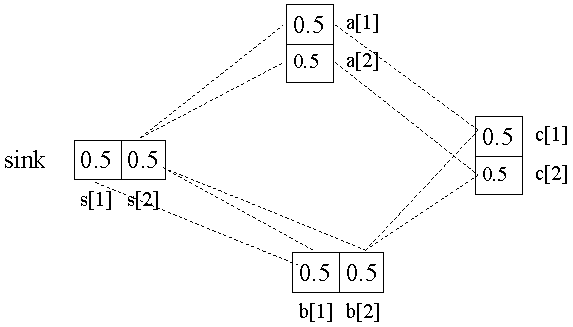
\includegraphics[width=2.75in]{4-node.pdf}
    \caption{An example network with locality sets}
    \label{fig:4node}
\vspace*{-0.25in}
    \end{center}
    \end{figure}
    % ------------------------------

\nwline
{\bf Example.}
     Fig.~\ref{fig:4node} illustrates a probabilistic graph on 4 nodes
     where $V= \{s, a,b,c\}$, and the locality set of each node has 2
     locations.
     %
     The network has $2^4$ states.
     %
     For the $\ACONN$ problem, 
     state $S_1= \{ s[2], a[2], b[2], c[2] \}$ is operating, and
     state $S_2= \{ s[1], a[1], b[1], c[2] \}$ is failed.
\IEEEQED
% ------------------------------
% ------------------------------------------------------------


